% Chapter Template

\chapter{Validació del sistema} % Main chapter title

Definits els components i detalls que componen el sistema de monitoratge i el sistema d'adaptabilitat, i un cop justificada des d'un punt de vista teòric la satisfacció dels nostres objectius, és el moment de presentar un exemple de cas d'ús i provar l'execució per validar el seu funcionament satisfactori i avaluar els resultats obtinguts.

\section{Presentació de cas d'ús}

Recordem la premissa genèrica del cas d'ús que volem que el nostre sistema satisfaci:

\begin{center}
\textit{Donada un \textbf{procés de monitoratge actiu} en un dels monitors del nostre sistema, i una proposta de \textbf{nova configuració} modelada, volem executar de forma automatitzada una \textbf{reconfiguració} d'aquell procés de monitoratge d'acord amb els \textbf{canvis computats respecte l'actual}.}
\end{center}

Per validar aquesta execució necessitem definir: un \textit{Base Model} que modeli l'estat actual del sistema (figura ~\ref{fig:Figura37}, una \textit{Feature Configuration} que modeli la darrera aplicada al sistema (figura ~\ref{fig:Figura37}, una \textit{Feature Configuration} que modeli la nova proposta de configuració del sistema (figura ~\ref{fig:Figura38}) i un \textit{Adaptability Model} que defineixi l'adaptació de models i la reconfiguració  de monitors (figura ~\ref{fig:Figura39}).

\begin{figure}
\centering
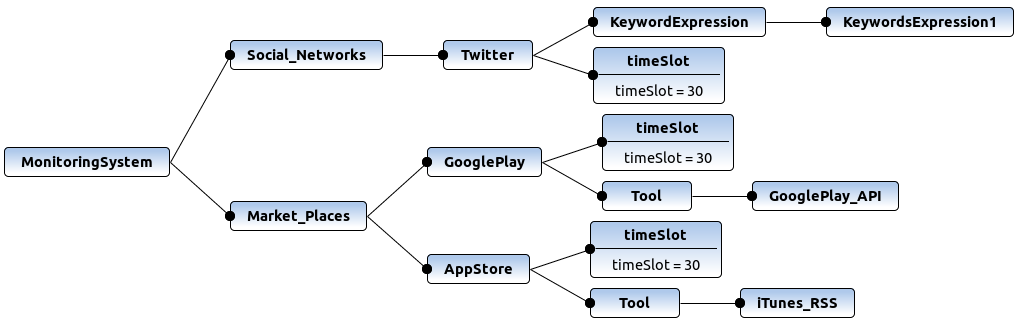
\includegraphics[width=14cm]{Figures/Figure36}
\decoRule
\caption{Disseny dels controladors REST del \textit{dashboard}}
\label{fig:Figura36}
\end{figure} 

\begin{figure}
\centering
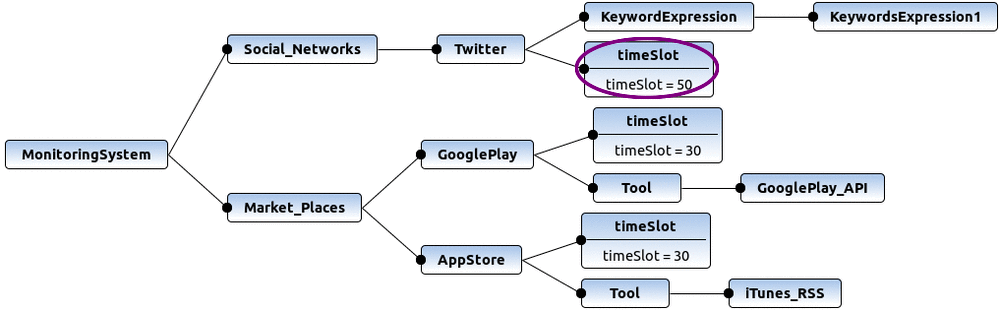
\includegraphics[width=14cm]{Figures/Figure37}
\decoRule
\caption{Disseny dels controladors REST del \textit{dashboard}}
\label{fig:Figura37}
\end{figure} 

\begin{figure}
\centering
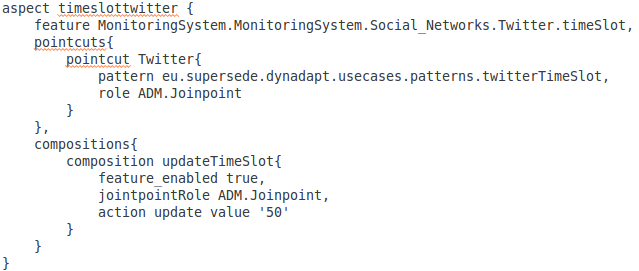
\includegraphics[width=14cm]{Figures/Figure38}
\decoRule
\caption{Disseny dels controladors REST del \textit{dashboard}}
\label{fig:Figura38}
\end{figure} 

\begin{figure}
\centering
\includegraphics[width=14cm]{Figures/Figure39}
\decoRule
\caption{Disseny dels controladors REST del \textit{dashboard}}
\label{fig:Figura39}
\end{figure} 

\section{Execució de la reconfiguració}